\documentclass[10pt]{article}
\usepackage{amsmath,amssymb,amsthm}
\usepackage{graphicx}
\usepackage[margin=1in]{geometry}
\usepackage[hidelinks]{hyperref}
\newtheorem{assumption}{Assumption}
\newtheorem{lemma}{Lemma}
\newtheorem{theorem}{Theorem}
\newtheorem{proposition}{Proposition}
\newtheorem{corollary}{Corollary}
\newcommand{\R}{\mathbb R}
\newcommand{\one}{\mathbf 1}
\DeclareMathOperator{\diag}{diag}
\DeclareMathOperator*{\argmin}{arg\,min}

\title{Linear Optimality and Constructive Nonlinear Improvement\\
for Positive Systems with Coupled Constraints}
\author{Anders Hansson}
\date{Research draft --- October 22, 2026}

\begin{document}
\maketitle

\begin{abstract}
We consider positive linear dynamics with linear stage costs and homogeneous convex constraints coupling states and controls. A finite conic program detects whether a globally admissible stationary linear feedback has finite cost everywhere and, when it does, computes a feedback minimizing cost in this class simultaneously for every initial state. Global optimality among arbitrary admissible policies is equivalent to a dual-cone condition and can be checked by minimizing the Bellman residual at any single strictly positive state. If the test fails, its optimizer gives an explicit nonlinear feedback using a scalar minimum. This feedback improves strictly on every globally admissible stationary linear feedback at every strictly positive initial state. The results do not require Bellman updates to preserve linear functions. For polyhedral constraints the programs are linear. Resource-conversion networks give an interpretation in terms of operations requiring several inventories. Examples establish linear optimality despite nonlinear intermediate Bellman iterates, an arbitrarily large cost of restricting feedback to be linear, and the absence of a general cost ordering between the explicit feedback and one-step rollout.
\end{abstract}

\section{Introduction}

Positive systems permit exact control computations that are difficult for general linear systems. Rantzer \cite{rantzer-2022} gave an explicit linear value for a positive-system class. Pates and Rantzer \cite{pates-rantzer} obtain linear value functions on positive cones when control minimization remains linear in the state. Their second theorem gives a dual characterization of that condition. Li and Rantzer \cite{li-rantzer} develop exact dynamic programming (DP) for positive systems with linear optimal cost. Li and Bertsekas \cite{li-bertsekas} study deterministic and stochastic problems in which Bellman updates preserve nonnegative linear functions and their minimizers belong to a specified class of policies. Blanchini and coauthors \cite{blanchini-2023} give an exact linear cost-to-go for a continuous-time compartmental control problem.

Coupled constraints also arise in network control. Ohlin, Tegling, and Rantzer \cite{ohlin-tegling-rantzer} give a linear programming (LP) solution and linear optimal feedback for positive networks with grouped input budgets. Arneson and Langbort \cite{arneson-langbort} give an LP characterization of optimal constant routing policies for a continuous-time network class. Ohlin, Rantzer, and Tegling \cite{ohlin-rantzer-tegling} give local control computations with performance bounds for their positive-network class. Mehrivash and Shafiei \cite{mehrivash-shafiei} use online LPs to control constrained positive systems while minimizing an upper bound on infinite-horizon linear cost. Schurig and coauthors \cite{schurig-2026} construct an admissible controller and performance bounds for fixed state and input capacities, where known explicit linear-value solutions do not apply. These works already establish linear feedback synthesis and bounded suboptimal control for important constrained positive systems.

Approximate DP includes lower bounds and policies computed from restricted value functions using Bellman inequalities \cite{de-farias-van-roy,wang-odonoghue-boyd}. Chakrabarty and coauthors \cite{chakrabarty-2019} incorporate state and input constraints into policy iteration using invariant sets for a quadratic-cost problem. Wang and Boyd \cite{wang-boyd-2011} study efficient evaluation of policies that minimize stage cost plus an approximate continuation value. For deterministic control, rollout uses the continuation cost of a feasible base policy and improves on that policy under general conditions \cite{li-johansson-martensson-bertsekas}. These precedents cover value approximation, constrained policy iteration, and policy improvement.

Explicit approximate control has additional precedents. Gutman and Cwikel \cite{gutman-cwikel} construct constrained stabilizing feedback from controls at vertices of a polyhedral state constraint set. Filippi \cite{filippi-2004} interpolates optimizers of parametric LPs to preserve feasibility and refines the partition to meet an objective-error tolerance. Bemporad and Filippi \cite{bemporad-filippi-2006} extend this approach to jointly convex parametric optimization. Jones and Morari \cite{jones-morari} construct feasible stabilizing controllers by interpolating controls over a polyhedral approximation of the optimal cost, without first computing the exact explicit controller. Rahal and coauthors \cite{rahal-2025} approximate parametric LP solutions using prescribed functions of the parameters built from affine functions and the scalar operation $s\mapsto\max\{s,0\}$. Thus feasible interpolation and simple explicit approximations are established methods.

Model predictive control (MPC) supplies further comparisons. Exact multiparametric LP converts a state-dependent LP controller into explicit feedback computed offline \cite{bemporad-borrelli-morari}. Approximate explicit MPC can reduce controller complexity while retaining feasibility and stability under sufficient conditions \cite{bemporad-filippi-2003,rubagotti-2012}. Hertneck and coauthors \cite{hertneck-2018} approximate robust MPC by supervised learning and obtain statistical guarantees of constraint satisfaction and stability. Ganguly and Chatterjee \cite{ganguly-2025} obtain uniform feedback-approximation guarantees and stability for nonlinear robust MPC using interpolation on a grid. Offline evaluation and certified approximation therefore do not distinguish the present result by themselves.

Here the state lies in the nonnegative orthant and the admissible state--control pairs form a closed convex cone with compact control sets at each state. We first compute the best stationary linear feedback that is admissible at every state and has finite cost. We then test its cost against all admissible actions at one strictly positive state. A zero minimum certifies global optimality; a negative minimum yields an explicit continuous piecewise linear feedback with a quantified strict cost reduction at every strictly positive state. The original Bellman operator need not preserve linear functions, and the test does not assume that the unrestricted value is linear.

The finite procedure combines synthesis of the best globally admissible stationary linear feedback, a global optimality test, and a nonlinear improvement when the test fails. Bellman updates preserve linear functions for the restricted controls by construction, as in the DP analysis of Li and Bertsekas \cite{li-bertsekas}. The optimality test uses the dual characterization of Pates and Rantzer \cite{pates-rantzer}. The nonlinear feedback is exactly the homogeneous extension of standard interpolation of rollout actions on a specified simplex partition \cite[Section~3.1]{bemporad-filippi-2006}. Its strict cost certificate follows from linearity of the residual and policy verification. The controller formula is therefore a specialization of established interpolation, and is not claimed as an independent new construction. The remaining contribution to assess is the combined optimality characterization for the stated conic control problem.

\section{Control problem and verification}

Vector inequalities are componentwise. Write $\R_+^n=\{x:x\ge0\}$ and $\R_{++}^n=\{x:x_i>0\text{ for every }i\}$. Let $e_i$ be the $i$th coordinate vector in $\R^n$, and let $\one$ denote a vector of ones of the indicated dimension. For a vector $a$, $\diag(a)$ is the diagonal matrix with entries $a_i$. A convex cone is a set closed under addition and multiplication by nonnegative scalars.

Fix $A\in\R^{n\times n}$, $B\in\R^{n\times m}$, $c\in\R^n$, $d\in\R^m$, and $0<\gamma\le1$. The dynamics, stage cost, and admissible controls are
\begin{equation}
 x_{t+1}=Ax_t+Bu_t,\qquad
 \ell(x,u)=c^\top x+d^\top u,\qquad
 U(x)=\{u:(x,u)\in G\}.
 \label{eq:problem}
\end{equation}

\begin{assumption}
\label{ass:data}
The set $G\subseteq\R_+^n\times\R^m$ is a closed convex cone. For every $x\ge0$, $U(x)$ is nonempty and compact. Every $(x,u)\in G$ satisfies $Ax+Bu\ge0$ and
\begin{equation}
 \ell(x,u)\ge\varepsilon\one^\top x
 \quad\text{for a fixed }\varepsilon>0.
 \label{eq:positive-cost}
\end{equation}
\end{assumption}

Assumption~\ref{ass:data} is imposed throughout. An admissible policy selects controls in $U(x_t)$ at every time, possibly using the preceding states and controls. Its cost and the optimal value are
\begin{equation}
 J^\pi(x)=\sum_{t=0}^{\infty}\gamma^t\ell(x_t,u_t),
 \quad x_0=x,\qquad
 J^*(x)=\inf_\pi J^\pi(x).
 \label{eq:cost}
\end{equation}
The sums in \eqref{eq:cost} may be infinite. A globally admissible stationary linear feedback is a matrix $K$ for which $(x,Kx)\in G$ for every $x\ge0$. Denote the set of such matrices by $\mathcal K$ and put
\begin{equation}
 M_K=A+BK,\qquad h_K=c+K^\top d,\qquad K\in\mathcal K.
 \label{eq:closed-loop}
\end{equation}
Assumption~\ref{ass:data} gives $M_K\ge0$ and $h_K\ge\varepsilon\one$. The spectral radius $\rho(M)$ is the largest absolute value of an eigenvalue of $M$.

\begin{lemma}
\label{lem:geometry}
The set $U(0)$ equals $\{0\}$, and
\begin{equation}
 K\in\mathcal K\quad\Longleftrightarrow\quad Ke_i\in U(e_i)
 \quad (i=1,\ldots,n).
 \label{eq:columns}
\end{equation}
\end{lemma}
\begin{proof}
The set $U(0)$ is a compact cone. A nonzero member would generate an unbounded ray, so $U(0)=\{0\}$. Necessity in \eqref{eq:columns} follows by evaluating feasibility at $e_i$. For sufficiency, use
\[
 (x,Kx)=\sum_{i=1}^n x_i(e_i,Ke_i)\in G,
 \qquad x\ge0,
\]
which holds by conic addition.
\end{proof}

\begin{lemma}
\label{lem:linear-cost}
For $K\in\mathcal K$, the cost $J^K$ is finite for every state if and only if $\gamma\rho(M_K)<1$. In that case
\begin{equation}
 J^K(x)=p_K^\top x,\qquad
 p_K=(I-\gamma M_K^\top)^{-1}h_K\ge\varepsilon\one.
 \label{eq:linear-cost}
\end{equation}
\end{lemma}
\begin{proof}
If $\gamma\rho(M_K)<1$, the convergent geometric matrix series gives
\[
 J^K(x)=\sum_{t=0}^\infty\gamma^t h_K^\top M_K^t x
 =h_K^\top(I-\gamma M_K)^{-1}x.
\]
Its coefficient is \eqref{eq:linear-cost}, and the first term of the nonnegative series gives $p_K\ge h_K\ge\varepsilon\one$.

Conversely, finiteness at every $e_i$ makes $p_K=\sum_{t\ge0}(\gamma M_K^\top)^t h_K$ a finite vector and gives $p_K=h_K+\gamma M_K^\top p_K$. Set $P_K=\diag(p_K)$ and $\eta_K=\varepsilon/\max_i(p_K)_i$. The $i$th row sum of the nonnegative matrix $P_K^{-1}\gamma M_K^\top P_K$ is
\[
 \frac{\gamma(M_K^\top p_K)_i}{(p_K)_i}
 =1-\frac{(h_K)_i}{(p_K)_i}
 \le1-\eta_K<1.
\]
Its spectral radius is bounded by its maximum row sum, so $\gamma\rho(M_K)<1$. The fixed-point equation now yields \eqref{eq:linear-cost}.
\end{proof}

For a coefficient vector $v\in\R^n$, define
\begin{align}
 V_v(x)&=v^\top x,\qquad
 \beta(v)=c+\gamma A^\top v-v,\qquad
 \nu(v)=d+\gamma B^\top v,\nonumber\\
 R_v(x,u)&=\ell(x,u)+\gamma V_v(Ax+Bu)-V_v(x)
           =\beta(v)^\top x+\nu(v)^\top u,\qquad
 q(v)=\begin{bmatrix}\beta(v)\\\nu(v)\end{bmatrix}.
 \label{eq:residual}
\end{align}
The dual cone of a cone $\mathcal H\subseteq\R^{n+m}$ is
\begin{equation}
 \mathcal H^\star=\{\xi\in\R^{n+m}:\xi^\top\zeta\ge0
       \text{ for every }\zeta\in\mathcal H\}.
 \label{eq:dual}
\end{equation}
In particular, $R_v\ge0$ on $G$ is equivalent to $q(v)\in G^\star$. The Bellman operator is
\begin{equation}
 (TV)(x)=\inf_{u\in U(x)}\{\ell(x,u)+\gamma V(Ax+Bu)\}.
 \label{eq:bellman}
\end{equation}

\begin{lemma}
\label{lem:verification}
Let $v\ge0$. If $R_v\ge0$ on $G$, then $V_v\le J^*$. If a stationary admissible feedback $\sigma$ satisfies $R_v(x,\sigma(x))\le0$ for all $x\ge0$, then $J^\sigma\le V_v$ and
\begin{equation}
 J^\sigma(x)=V_v(x)+\sum_{t=0}^\infty\gamma^tR_v(x_t,\sigma(x_t)).
 \label{eq:performance-identity}
\end{equation}
If both residual conditions hold, $J^*=J^\sigma=V_v$.
\end{lemma}
\begin{proof}
For every admissible trajectory and $N\ge1$, summing \eqref{eq:residual} gives
\begin{equation}
 \sum_{t=0}^{N-1}\gamma^t\ell(x_t,u_t)
 =V_v(x_0)-\gamma^NV_v(x_N)
   +\sum_{t=0}^{N-1}\gamma^tR_v(x_t,u_t).
 \label{eq:telescoping}
\end{equation}
Along a finite-cost trajectory, \eqref{eq:positive-cost} implies
\begin{equation}
 0\le\gamma^N\|x_N\|_1
 \le\varepsilon^{-1}\gamma^N\ell(x_N,u_N)\longrightarrow0.
 \label{eq:tail}
\end{equation}
Thus $\gamma^NV_v(x_N)\to0$. When $R_v\ge0$, \eqref{eq:telescoping} gives $V_v(x_0)$ as a lower bound on every finite cost after taking $N\to\infty$. Infinite costs satisfy the same bound, proving $V_v\le J^*$.

Under $\sigma$, the residual terms in \eqref{eq:telescoping} are nonpositive and the terminal value is nonnegative. Every partial cost is therefore at most $V_v(x_0)$. The nonnegative partial costs converge to a finite cost. Equation~\eqref{eq:tail} applies, and passage to the limit in \eqref{eq:telescoping} proves \eqref{eq:performance-identity}. Combining the lower and upper bounds proves the last statement.
\end{proof}

\section{The best globally admissible stationary linear feedback}

Define the coordinate control sets and their state-dependent sums by
\begin{equation}
 U_i=U(e_i),\qquad
 U_{\rm lin}(x)=\left\{\sum_{i=1}^n x_i v_i:v_i\in U_i\right\},\qquad
 G_{\rm lin}=\{(x,u):x\ge0,\ u\in U_{\rm lin}(x)\}.
 \label{eq:restriction}
\end{equation}
Each $U_i$ is nonempty and compact. Lemma~\ref{lem:geometry} gives
\begin{equation}
 U_{\rm lin}(x)=\{Kx:K\in\mathcal K\}\subseteq U(x).
 \label{eq:all-linear-actions}
\end{equation}
The set $G_{\rm lin}$ is a convex cone: to add two decompositions in \eqref{eq:restriction}, combine their $i$th controls by convex weights proportional to the corresponding state coordinates. If their sum is zero, that coordinate contributes zero. It is closed: for a convergent sequence of pairs, select a convergent subsequence of their control tuples in the compact product $U_1\times\cdots\times U_n$ and pass to the limit in \eqref{eq:restriction}.

Let $J_{\rm lin}$ be the optimal value when admissible actions are restricted to $U_{\rm lin}(x)$ in \eqref{eq:restriction} at every time. This restriction still permits history-dependent policies. We say that a Bellman operator has linear Bellman closure if it sends every nonnegative linear function to a linear function. Define the coefficient update $\Phi:\R_+^n\to\R_+^n$ by
\begin{equation}
 \Phi(v)_i=c_i+\gamma(A^\top v)_i
       +\min_{a\in U_i}\nu(v)^\top a.
 \label{eq:coefficient-update}
\end{equation}
The minimum in \eqref{eq:coefficient-update} exists by compactness. Nonnegativity follows from
\[
 \Phi(v)_i=\min_{a\in U_i}\{\ell(e_i,a)+\gamma v^\top(Ae_i+Ba)\}\ge0.
\]
Separation of the coordinates gives
\begin{equation}
 \min_{u\in U_{\rm lin}(x)}\{\ell(x,u)+\gamma V_v(Ax+Bu)\}
 =\Phi(v)^\top x.
 \label{eq:restricted-bellman}
\end{equation}

\begin{theorem}
\label{thm:best-linear}
Suppose some $K_0\in\mathcal K$ satisfies $\gamma\rho(M_{K_0})<1$. The iteration $p^{(0)}=0$, $p^{(k+1)}=\Phi(p^{(k)})$ converges to a vector $p\ge\varepsilon\one$. There is $K_{\rm lin}\in\mathcal K$ such that
\begin{equation}
 J_{\rm lin}(x)=J^{K_{\rm lin}}(x)=p^\top x\le J^K(x)
 \quad(x\ge0,\ K\in\mathcal K).
 \label{eq:best-linear}
\end{equation}
The columns of $K_{\rm lin}$ can be chosen independently as
\begin{equation}
 K_{\rm lin}e_i\in\argmin_{a\in U_i}\nu(p)^\top a.
 \label{eq:optimal-columns}
\end{equation}
The vector $p$ is the largest element, in componentwise order, of
\begin{equation}
 \mathcal P_{\rm lin}=\{v\ge0:q(v)\in G_{\rm lin}^\star\}.
 \label{eq:restricted-subsolutions}
\end{equation}
\end{theorem}
\begin{proof}
Positivity of successors shows that $v\le\widehat v$ implies $\Phi(v)\le\Phi(\widehat v)$. Also $\Phi(0)\ge\varepsilon\one$. Thus the iterates increase componentwise. By Lemma~\ref{lem:linear-cost}, $p_{K_0}$ is finite. Evaluating each minimum in \eqref{eq:coefficient-update} at $K_0e_i$ gives $\Phi(p_{K_0})\le p_{K_0}$. Induction yields $0\le p^{(k)}\le p_{K_0}$, so the iterates converge to a finite vector $p\ge\varepsilon\one$.

For each $i$, set $L_i=\max_{a\in U_i}\|Ae_i+Ba\|_2<\infty$. Taking differences between the minima defining $\Phi$ gives
\[
 |\Phi(v)_i-\Phi(\widehat v)_i|
 \le\gamma L_i\|v-\widehat v\|_2.
\]
Consequently $p=\Phi(p)$. Choose the columns in \eqref{eq:optimal-columns}; Lemma~\ref{lem:geometry} makes $K_{\rm lin}$ globally admissible. The fixed-point equation gives
\begin{equation}
 p=h_{K_{\rm lin}}+\gamma M_{K_{\rm lin}}^\top p,
 \qquad R_p(x,K_{\rm lin}x)=0.
 \label{eq:linear-equality}
\end{equation}
The row-sum argument in the proof of Lemma~\ref{lem:linear-cost}, applied to \eqref{eq:linear-equality}, gives $\gamma\rho(M_{K_{\rm lin}})<1$ and $p=p_{K_{\rm lin}}$.

Equations~\eqref{eq:restricted-bellman} and \eqref{eq:linear-equality} imply $R_p\ge0$ on $G_{\rm lin}$. Lemma~\ref{lem:verification}, applied to this restricted set of admissible pairs, gives $V_p\le J_{\rm lin}$. The feedback $K_{\rm lin}$ attains $V_p$, so $J_{\rm lin}=V_p$. Every globally admissible stationary linear feedback uses actions in \eqref{eq:all-linear-actions}, proving \eqref{eq:best-linear}, including feedbacks of infinite cost.

Finally, $v\in\mathcal P_{\rm lin}$ means $R_v\ge0$ on $G_{\rm lin}$ by \eqref{eq:restricted-subsolutions}, \eqref{eq:dual}, and \eqref{eq:residual}. Lemma~\ref{lem:verification}, applied to the restricted controls, gives $v^\top x\le J_{\rm lin}(x)=p^\top x$. Evaluation at every $e_i$ yields $v\le p$. Since $p\in\mathcal P_{\rm lin}$ by \eqref{eq:restricted-bellman} and $p=\Phi(p)$, it is the largest element.
\end{proof}

The restricted problem in \eqref{eq:restriction} satisfies linear Bellman closure, the property used in the DP analysis of \cite{li-bertsekas}. Theorem~\ref{thm:best-linear} does not assert linear Bellman closure for the original controls in \eqref{eq:problem}. It also bounds the cost of time-dependent globally admissible linear gains, since those policies remain admissible for the restricted problem.

Fix $w\in\R_{++}^n$. Introduce $z\in\R^n$ and $y_i\in\R^m$, and consider the finite conic program
\begin{equation}
 \begin{array}{ll}
 \operatorname{minimize}_{z,y_1,\ldots,y_n}
     &c^\top z+d^\top\displaystyle\sum_i y_i\\[1mm]
 \operatorname{subject\ to}
     &z=w+\gamma\left(Az+B\displaystyle\sum_i y_i\right),\\
     &(z_i e_i,y_i)\in G,\qquad i=1,\ldots,n.
 \end{array}
 \label{eq:synthesis}
\end{equation}

\begin{theorem}
\label{thm:synthesis}
Program~\eqref{eq:synthesis} is feasible if and only if some $K\in\mathcal K$ has finite cost at every state. When feasible, it attains the value $p^\top w$, where $p$ is from Theorem~\ref{thm:best-linear}. Every optimizer satisfies $z\ge w>0$ and recovers a globally admissible stationary linear feedback of cost $p^\top x$ through
\begin{equation}
 Ke_i=y_i/z_i,\qquad i=1,\ldots,n.
 \label{eq:recovery}
\end{equation}
\end{theorem}
\begin{proof}
For a feasible point, each successor $Az_i e_i+By_i$ is nonnegative. The balance constraint in \eqref{eq:synthesis} therefore gives $z\ge w>0$. Conic scaling and Lemma~\ref{lem:geometry} make \eqref{eq:recovery} globally admissible. The balance constraint becomes $\gamma M_Kz=z-w$. All row sums of $\diag(z)^{-1}\gamma M_K\diag(z)$ are $1-w_i/z_i<1$, proving $\gamma\rho(M_K)<1$. Thus
\[
 z=(I-\gamma M_K)^{-1}w,\qquad
 c^\top z+d^\top\sum_i y_i=h_K^\top z=J^K(w).
\]
Conversely, for any globally admissible $K$ of finite cost, take $z=(I-\gamma M_K)^{-1}w$ and $y_i=z_iKe_i$. Then $z\ge w$, each $(z_i e_i,y_i)$ belongs to $G$, and the balance constraint holds. Its objective is $J^K(w)$.

Feasibility now permits Theorem~\ref{thm:best-linear}. Using $K_{\rm lin}$ in the converse construction attains $p^\top w$, and every feasible point has objective $J^K(w)\ge p^\top w$. For an optimizer, Lemma~\ref{lem:linear-cost} and \eqref{eq:best-linear} give $p_K\ge p$ and $(p_K-p)^\top w=0$. Since $w_i>0$ for every $i$, each component of $p_K-p$ is zero. Hence the recovered feedback has cost $p^\top x$ at every state.
\end{proof}

Infeasibility of \eqref{eq:synthesis} only excludes globally admissible stationary linear feedback with finite cost everywhere. It does not exclude successful nonlinear feedback. The remainder of the paper assumes that \eqref{eq:synthesis} is feasible, and uses the fixed $p$ and $K_{\rm lin}$ from Theorem~\ref{thm:best-linear}.

\section{Global optimality and nonlinear improvement}

At the strictly positive state $w$, define the minimized residual
\begin{equation}
 r_w=\min_{u\in U(w)}R_p(w,u).
 \label{eq:interior-test}
\end{equation}
The minimum is attained because $U(w)$ is compact. Equation~\eqref{eq:linear-equality} gives $r_w\le0$.

\begin{theorem}
\label{thm:exactness}
The following statements are equivalent:
\begin{enumerate}
 \item $r_w=0$.
 \item $q(p)\in G^\star$.
 \item $K_{\rm lin}$ is optimal among all admissible policies at every state.
 \item $J^*$ is a linear function on $\R_+^n$.
\end{enumerate}
When they hold, $J^*(x)=p^\top x$ for every $x\ge0$.
\end{theorem}
\begin{proof}
Suppose $r_w=0$ but $q(p)\notin G^\star$. By \eqref{eq:dual}, there is $(\widehat x,\widehat u)\in G$ with $R_p(\widehat x,\widehat u)<0$. Lemma~\ref{lem:geometry} excludes $\widehat x=0$. Choose $\tau>0$ with $w-\tau\widehat x\ge0$. Conic addition gives
\[
 (w,\tau\widehat u+K_{\rm lin}(w-\tau\widehat x))\in G.
\]
Linearity of \eqref{eq:residual} and \eqref{eq:linear-equality} give residual $\tau R_p(\widehat x,\widehat u)<0$ at this pair, contradicting $r_w=0$. This proves $1\Rightarrow2$. Conversely, $q(p)\in G^\star$ gives $r_w\ge0$, and $r_w\le0$ was already established.

Statement 2 and \eqref{eq:linear-equality} imply statement 3 and $J^*=V_p$ by Lemma~\ref{lem:verification}. Statement 3 implies statement 4 by \eqref{eq:best-linear}.

Suppose statement 4 holds, and write $J^*=V_b$ for some vector $b$. Since every trajectory pays its first stage cost, \eqref{eq:positive-cost} gives $b\ge\varepsilon\one$. Finiteness of $J^*$ follows from the available $K_{\rm lin}$. Splitting an admissible trajectory after its first action gives $J^*\ge TJ^*$. Conversely, for any first action, append a trajectory whose cost is within an arbitrary positive tolerance of the successor value. Taking the infimum over first actions and then letting the tolerance tend to zero gives $J^*\le TJ^*$. Thus $J^*=TJ^*$.

At $e_i$, compactness of $U_i$ gives a minimizing control $a_i$ in this Bellman equation. Let $\widehat K e_i=a_i$. Lemma~\ref{lem:geometry} gives $\widehat K\in\mathcal K$, and
\[
 R_b(e_i,a_i)=0\quad\text{for every }i,
 \qquad R_b(x,\widehat Kx)=\sum_i x_iR_b(e_i,a_i)=0.
\]
The Bellman equation also gives $R_b\ge0$ on $G$. Lemma~\ref{lem:verification} shows that $\widehat K$ has finite cost $J^{\widehat K}=J^*$. Since it is admissible for the restricted problem, $J_{\rm lin}\le J^{\widehat K}=J^*$. The inclusion in \eqref{eq:all-linear-actions} gives $J^*\le J_{\rm lin}$. Hence $J^*=J_{\rm lin}=V_p$, so $b=p$ and $q(p)\in G^\star$.
\end{proof}

Theorem~\ref{thm:exactness} also implies that a globally optimal stationary linear feedback exists if and only if the four statements hold: its finite cost is linear by Lemma~\ref{lem:linear-cost}. The role of $w>0$ is essential to the extension of a residual violation to the tested state.

When $r_w<0$, choose a minimizing $\bar u\in U(w)$ and define
\begin{equation}
 \delta=-r_w>0,\qquad
 \theta(x)=\min_{1\le i\le n}\frac{x_i}{w_i},\qquad
 \mu(x)=K_{\rm lin}x+\theta(x)(\bar u-K_{\rm lin}w).
 \label{eq:improved-feedback}
\end{equation}

\begin{theorem}
\label{thm:improvement}
If $r_w<0$, the feedback $\mu$ in \eqref{eq:improved-feedback} is globally admissible and has finite cost everywhere. Along its trajectory,
\begin{equation}
 J^\mu(x)=p^\top x-\delta\sum_{t=0}^\infty\gamma^t\theta(x_t)
 \le p^\top x-\delta\theta(x).
 \label{eq:strict-gain}
\end{equation}
In particular, $J^\mu(x)<J^K(x)$ for every $x\in\R_{++}^n$ and every $K\in\mathcal K$. If $\gamma=1$, the origin is globally exponentially stable under $\mu$.
\end{theorem}
\begin{proof}
The definition of $\theta$ gives $x-\theta(x)w\ge0$. Thus
\[
 (x,\mu(x))=\theta(x)(w,\bar u)
 +(x-\theta(x)w,K_{\rm lin}(x-\theta(x)w))\in G.
\]
Using \eqref{eq:linear-equality} and $R_p(w,\bar u)=-\delta$ yields
\begin{equation}
 R_p(x,\mu(x))=-\delta\theta(x)\le0.
 \label{eq:improvement-residual}
\end{equation}
Lemma~\ref{lem:verification} proves finiteness and \eqref{eq:strict-gain}. At $x>0$, every ratio $x_i/w_i$ is positive, so $\theta(x)>0$. Combining \eqref{eq:strict-gain} with \eqref{eq:best-linear} proves strict improvement over every $K\in\mathcal K$.

For $\gamma=1$, let $p_{\min}=\min_i p_i$, $p_{\max}=\max_i p_i$, and $\eta=\varepsilon/p_{\max}\in(0,1]$. Equations~\eqref{eq:positive-cost} and \eqref{eq:improvement-residual} give
\[
 p^\top x_{t+1}\le p^\top x_t-\varepsilon\|x_t\|_1
 \le(1-\eta)p^\top x_t.
\]
If $\eta<1$, iteration gives $\|x_t\|_1\le(p_{\max}/p_{\min})(1-\eta)^t\|x_0\|_1$. If $\eta=1$, the next state is zero because $p>0$ and $x_{t+1}\ge0$. Both cases give global exponential stability.
\end{proof}

The feedback in \eqref{eq:improved-feedback} is continuous and piecewise linear on at most $n$ regions defined by linear inequalities, one for each ratio that can attain the minimum in $\theta$. Its evaluation requires no online optimization. Theorem~\ref{thm:improvement} does not assert that $\mu$ is optimal among nonlinear feedbacks. For $\gamma<1$, finite discounted cost does not by itself imply convergence of the state to zero.

For comparison, one-step rollout from $K_{\rm lin}$ selects $\mu_{\rm roll}(x)\in\arg\min_{u\in U(x)}R_p(x,u)$ at each state, since $J^{K_{\rm lin}}=V_p$. A minimizer exists by Assumption~\ref{ass:data}. Global admissibility of $\mu$ and \eqref{eq:improvement-residual} give
\[
 R_p(x,\mu_{\rm roll}(x))\le R_p(x,\mu(x))=-\delta\theta(x)\le0.
\]
Lemma~\ref{lem:verification} and \eqref{eq:performance-identity} give
\[
 J^{\mu_{\rm roll}}(x)=p^\top x+\sum_{t=0}^\infty\gamma^tR_p(x_t,\mu_{\rm roll}(x_t))
 \le p^\top x+R_p(x,\mu_{\rm roll}(x))
 \le p^\top x-\delta\theta(x).
\]
The bound is strict when $x>0$, so rollout has the same strict-improvement guarantee \cite{li-johansson-martensson-bertsekas}. The distinction of \eqref{eq:improved-feedback} is that it uses one offline minimizer $\bar u$ at $w$ and evaluates only $\theta(x)$ online. Equations~\eqref{eq:strict-gain} and \eqref{eq:performance-identity} do not order $J^{\mu_{\rm roll}}$ and $J^\mu$.

\subsection{Exact relation to interpolation of rollout actions}

A simplex is the convex hull of affinely independent points. Assume $n\ge2$ and $r_w<0$, and define
\begin{equation}
 \Delta=\{x\ge0:\one^\top x=1\},\qquad
 \Delta_i=\operatorname{conv}\left(\left\{\frac{w}{\one^\top w}\right\}
       \cup\{e_j:j\ne i\}\right),\quad i=1,\ldots,n.
 \label{eq:interpolation-partition}
\end{equation}
Here $\operatorname{conv}$ denotes all convex combinations of the indicated points. Each $\Delta_i$ has dimension $n-1$. Interpolation on such a simplex assigns the same convex weights to the controls prescribed at its vertices. This is the construction in \cite{filippi-2004} and \cite[Section~3.1, Proposition~3.1]{bemporad-filippi-2006}. Eliminating the last state coordinate makes $\Delta$ full dimensional in $\R^{n-1}$, as required for their parameterization.

\begin{proposition}
\label{prop:interpolation}
The sets $\Delta_i$ in \eqref{eq:interpolation-partition} cover $\Delta$ and meet along shared faces. The controls $K_{\rm lin}e_j$ and $\bar u/(\one^\top w)$ minimize the rollout residual at $e_j$ and $w/(\one^\top w)$, respectively. Interpolating these controls on each $\Delta_i$ and extending by positive homogeneity gives exactly $\mu$ in \eqref{eq:improved-feedback}.
\end{proposition}
\begin{proof}
For $x\in\Delta$, choose an index $i$ attaining the minimum in \eqref{eq:improved-feedback}. Define the weights
\begin{equation}
 \omega_0(x)=\theta(x)\one^\top w,\qquad
 \omega_j(x)=x_j-\theta(x)w_j\quad(j=1,\ldots,n).
 \label{eq:interpolation-weights}
\end{equation}
They are nonnegative, $\omega_i(x)=0$, and
\[
 \omega_0(x)+\sum_{j\ne i}\omega_j(x)=\one^\top x=1,\qquad
 \omega_0(x)\frac{w}{\one^\top w}
       +\sum_{j\ne i}\omega_j(x)e_j=x.
\]
Thus $x\in\Delta_i$. Conversely, if $x\in\Delta_i$, its coefficient on $w/(\one^\top w)$ is $x_i\one^\top w/w_i$, and nonnegativity of the remaining coefficients gives $x_j/w_j\ge x_i/w_i$ for every $j$. Hence
\[
 \Delta_i=\{x\in\Delta:x_i/w_i\le x_j/w_j\text{ for all }j\}.
\]
The coordinate vertices with $j\ne i$ lie in $x_i=0$, whereas $w_i>0$; they are affinely independent with $w/(\one^\top w)$. The weights are therefore unique. A tie between indices $i$ and $k$ sets both corresponding weights to zero, so the intersection is their shared face. These facts prove the partition assertion.

Equations~\eqref{eq:restriction}, \eqref{eq:optimal-columns}, and \eqref{eq:linear-equality} give
\[
 \min_{u\in U(e_j)}R_p(e_j,u)
 =R_p(e_j,K_{\rm lin}e_j)=0.
\]
For every scalar $a>0$, conic scaling in both directions gives $U(ax)=aU(x)$. Linearity of \eqref{eq:residual} therefore shows that $\bar u/(\one^\top w)$ minimizes the residual at $w/(\one^\top w)$. Its residual is $r_w/(\one^\top w)$.

On $\Delta_i$, the interpolated action is
\begin{align*}
 \omega_0(x)\frac{\bar u}{\one^\top w}
 +\sum_{j\ne i}\omega_j(x)K_{\rm lin}e_j
 &=\theta(x)\bar u+K_{\rm lin}(x-\theta(x)w)\\
 &=\mu(x).
\end{align*}
The weights for a tied index vanish, so the interpolants agree on shared faces. For nonzero $x\ge0$, apply this equality at $x/(\one^\top x)$ and multiply by $\one^\top x$; positive homogeneity of \eqref{eq:improved-feedback} gives the equality at $x$. Both controls are zero at the origin by Lemma~\ref{lem:geometry}.
\end{proof}

The specialization is exact, including the residual certificate. On $\Delta_i$, linearity of \eqref{eq:residual} and the vertex residuals in Proposition~\ref{prop:interpolation} give
\[
 R_p(x,\mu(x))
 =\omega_0(x)\frac{r_w}{\one^\top w}+\sum_{j\ne i}\omega_j(x)\,0
 =-\delta\theta(x).
\]
Positive homogeneity extends this equality to the orthant, recovering \eqref{eq:improvement-residual}. Lemma~\ref{lem:verification} then gives \eqref{eq:strict-gain}. Thus standard interpolation with the prescribed vertices recovers the controller, its region count, and, together with policy verification, its strict cost certificate. This does not assert that the adaptive subdivision algorithms in the cited papers select these particular vertices or stop at this partition for a prescribed approximation tolerance. For nonpolyhedral $G$, the interpolation proof still applies directly by convexity, without requiring the finite differentiable constraint descriptions used by those algorithms. For $n=1$, conic scaling gives $U(x)=xU(e_1)$ for $x>0$; \eqref{eq:all-linear-actions} is then an equality, and $r_w<0$ cannot occur.

\begin{corollary}
\label{cor:one-state}
There exists a globally admissible stationary linear feedback that is optimal among all admissible policies at some strictly positive initial state if and only if $K_{\rm lin}$ is globally optimal.
\end{corollary}
\begin{proof}
If $K\in\mathcal K$ is optimal at a strictly positive state $x$, its cost there is finite. Since $e_i\le x/x_i$ and $M_K,h_K\ge0$ by \eqref{eq:closed-loop} and Assumption~\ref{ass:data}, every partial cost satisfies
\[
 \sum_{t=0}^{N-1}\gamma^t h_K^\top M_K^t e_i
 \le\frac{1}{x_i}\sum_{t=0}^{N-1}\gamma^t h_K^\top M_K^t x
 \le\frac{J^K(x)}{x_i}.
\]
Thus $J^K(e_i)$ is finite for each $i$, and Lemma~\ref{lem:linear-cost} applies. If $r_w<0$, Theorem~\ref{thm:improvement} would strictly improve its cost at $x$, a contradiction. Thus $r_w=0$, and Theorem~\ref{thm:exactness} gives global optimality of $K_{\rm lin}$. The converse follows from global optimality of $K_{\rm lin}$.
\end{proof}

If $K\in\mathcal K$ is optimal at a strictly positive state, then $p_K\ge p$ by \eqref{eq:best-linear}; equality of cost at that state gives $p_K=p$ componentwise. Thus $J^K(x)=p^\top x$ for every $x\ge0$ by \eqref{eq:linear-cost}.

\section{Finite LP formulas and a performance bound}

Suppose the cone has the polyhedral description
\begin{equation}
 G=\{(x,u):x\ge0,\ F x+Hu\ge0\},
 \qquad F\in\R^{r\times n},\ H\in\R^{r\times m}.
 \label{eq:polyhedral}
\end{equation}
Then the conic constraints in \eqref{eq:synthesis} are exactly $z_i\ge0$ and $F e_i z_i+Hy_i\ge0$. Hence \eqref{eq:synthesis} is an LP with $n+nm$ variables. An alternative LP computes $p$ directly:
\begin{equation}
 \begin{array}{ll}
 \operatorname{maximize}_{v,\lambda_1,\ldots,\lambda_n}&w^\top v\\
 \operatorname{subject\ to}&v\ge0,\quad\lambda_i\ge0,\\
 &H^\top\lambda_i=\nu(v),\quad
   (F e_i)^\top\lambda_i\le\beta(v)_i,
   \qquad i=1,\ldots,n.
 \end{array}
 \label{eq:coefficient-lp}
\end{equation}

\begin{proposition}
\label{prop:lp}
Under \eqref{eq:polyhedral}, the unique optimal coefficient in \eqref{eq:coefficient-lp} is $p$. The condition $q(p)\in G^\star$ is equivalent to feasibility of
\begin{equation}
 \lambda\ge0,\qquad H^\top\lambda=\nu(p),\qquad
 F^\top\lambda\le\beta(p).
 \label{eq:common-dual}
\end{equation}
Every feasible $\lambda$ in \eqref{eq:common-dual} satisfies $F^\top\lambda=\beta(p)$.
\end{proposition}
\begin{proof}
The coordinate set is $U_i=\{a:Ha\ge-F e_i\}$. LP duality \cite[Chapter~5]{boyd-vandenberghe}, together with its nonempty compact feasible set, gives
\begin{equation}
 \min_{a\in U_i}\nu(v)^\top a
 =\max_{\lambda_i\ge0,\ H^\top\lambda_i=\nu(v)}
       -(F e_i)^\top\lambda_i,
 \label{eq:coordinate-dual}
\end{equation}
with attainment on both sides. The inequality $\beta(v)_i+\min_{a\in U_i}\nu(v)^\top a\ge0$ is therefore equivalent to the existence of $\lambda_i$ satisfying the $i$th constraints in \eqref{eq:coefficient-lp}. By \eqref{eq:restricted-bellman}, these inequalities characterize $q(v)\in G_{\rm lin}^\star$. Theorem~\ref{thm:best-linear} shows $v\le p$ for every feasible $v$ and feasibility of $p$. Since $w>0$, equality $w^\top v=w^\top p$ forces $v=p$.

Farkas' lemma gives
\[
 G^\star=\left\{\begin{bmatrix}s+F^\top\lambda\\H^\top\lambda\end{bmatrix}:
                 s\ge0,\ \lambda\ge0\right\},
\]
which proves the equivalence with \eqref{eq:common-dual}. To prove equality in its last constraint, the fixed-point equation $p=\Phi(p)$ gives $\beta(p)_i=-\min_{a\in U_i}\nu(p)^\top a$. For a feasible common $\lambda$, weak duality in \eqref{eq:coordinate-dual} yields $\beta(p)_i\le(F e_i)^\top\lambda$. The reverse inequality is part of \eqref{eq:common-dual}, proving equality for every component.
\end{proof}

The LP in \eqref{eq:coefficient-lp} permits a different multiplier for each coordinate state. Exactness requires a single multiplier satisfying all coordinates at once, as in \eqref{eq:common-dual}. Both conditions use standard LP duality. Requiring one multiplier in \eqref{eq:common-dual} specializes the dual characterization in \cite[Theorem~2]{pates-rantzer} at the computed continuation coefficient $\nu(p)$. Their Theorem~1 requires control minimization to be linear in the state for every control coefficient covered by its dual-cone hypothesis. Polyhedrality alone does not ensure that property. Our exactness test concerns only $\nu(p)$.

For a general nonpolyhedral $G$, \eqref{eq:synthesis} and \eqref{eq:interior-test} are finite conic programs when membership in $G$ has a finite conic description. Their mathematical conclusions do not require a strict-feasibility assumption. Numerical conic implementations may still need to account for the boundary constraints $(z_i e_i,y_i)\in G$.

A quantitative bound is available even when exactness fails. Define
\begin{equation}
 \kappa=\min\left\{\kappa_0\ge1:
 \begin{bmatrix}\kappa_0 c+\gamma A^\top p-p\\\kappa_0 d+\gamma B^\top p\end{bmatrix}
 \in G^\star\right\}.
 \label{eq:factor}
\end{equation}

\begin{proposition}
\label{prop:factor}
The minimum in \eqref{eq:factor} is finite and attained. For every $x\ge0$,
\begin{equation}
 \kappa^{-1}p^\top x\le J^*(x)\le p^\top x.
 \label{eq:factor-bound}
\end{equation}
Furthermore, $\kappa=1$ if and only if the equivalent conditions of Theorem~\ref{thm:exactness} hold. Under \eqref{eq:polyhedral}, \eqref{eq:factor} is an LP.
\end{proposition}
\begin{proof}
For any admissible pair, $p^\top(Ax+Bu)\ge0$ and
\[
 p^\top x-\gamma p^\top(Ax+Bu)
 \le(\max_i p_i)\|x\|_1
 \le\frac{\max_i p_i}{\varepsilon}\ell(x,u).
\]
Thus $\kappa_0=(\max_i p_i)/\varepsilon\ge1$ is feasible. The feasible set in \eqref{eq:factor} is closed because $G^\star$ is closed, so the finite infimum is attained. Dividing its defining inequality by $\kappa$ gives $R_{p/\kappa}\ge0$ on $G$. Lemma~\ref{lem:verification} proves the lower bound; the policy $K_{\rm lin}$ proves the upper bound. At $\kappa_0=1$, the condition in \eqref{eq:factor} is exactly $q(p)\in G^\star$, proving the equivalence. The polyhedral dual formula used in Proposition~\ref{prop:lp} makes \eqref{eq:factor} an LP in $\kappa_0$ and its nonnegative multipliers.
\end{proof}

These results give a finite procedure: solve \eqref{eq:synthesis}, recover a best linear feedback with \eqref{eq:recovery}, and compute its coefficient with \eqref{eq:linear-cost}. Solve \eqref{eq:interior-test}. A zero optimum certifies global optimality by Theorem~\ref{thm:exactness}; a negative optimum supplies \eqref{eq:improved-feedback}. Program~\eqref{eq:factor} supplies the additional bound \eqref{eq:factor-bound}. All exactness statements concern exact feasibility and equality; floating-point tolerances alone do not establish these equalities.

\section{Resource-conversion networks}

Let $A_0\in\R_+^{n\times n}$ and $C,D\in\R_+^{n\times m}$, with every column of $C$ nonzero. Specialize \eqref{eq:problem} to
\begin{equation}
 x^+=A_0(x-Cu)+Du,\qquad u\ge0,\quad Cu\le x,
 \qquad c\in\R_{++}^n,\quad d\ge0.
 \label{eq:resource}
\end{equation}
Thus the original matrices satisfy $A=A_0$ and $B=D-A_0C$. The vector $x$ records available resources. Column $C_j$ specifies the resources consumed per unit of operation $j$, and column $D_j$ its outputs. Unprocessed resources evolve under $A_0$. These are homogeneous regulation or depletion dynamics, without external arrivals or fixed capacity bounds.

The constraints in \eqref{eq:resource} define a closed convex cone with a nonempty control set at every state, since $u=0$ is feasible. For each operation $j$, select an index $i$ with $C_{ij}>0$. Then $0\le u_j\le x_i/C_{ij}$, proving compactness. Positivity of the successor follows from $x-Cu\ge0$, and \eqref{eq:positive-cost} holds with $\varepsilon=\min_i c_i$. Thus Assumption~\ref{ass:data} holds.

Let $f_j$ be the $j$th coordinate vector in $\R^m$, and define
\begin{equation}
 \chi_j=d_j+c^\top C_j+\gamma p^\top D_j-p^\top C_j,
 \qquad j=1,\ldots,m.
 \label{eq:operation-test}
\end{equation}

\begin{proposition}
\label{prop:resource}
For \eqref{eq:resource}, every $K\in\mathcal K$ has a zero $j$th row whenever $C_j$ has at least two positive entries. Subject to feasibility of \eqref{eq:synthesis}, global optimality of $K_{\rm lin}$ is equivalent to $\chi_j\ge0$ for every $j$. If $\chi_j<0$, using $u=f_j$ at $x=C_j$ and then following $K_{\rm lin}$ has cost $p^\top C_j+\chi_j<p^\top C_j$.
\end{proposition}
\begin{proof}
Global feasibility in \eqref{eq:resource} is equivalent to $K\ge0$ and $CK\le I$. Fix an operation $j$ whose consumption column has two positive entries. For any state coordinate $k$, choose $i\ne k$ with $C_{ij}>0$. Then
\[
 0\le C_{ij}K_{jk}\le(CK)_{ik}\le I_{ik}=0.
\]
Hence $K_{jk}=0$ for every $k$, proving the row statement.

The control $0$ belongs to every $U_i$. Since $p=\Phi(p)$, evaluating the coordinate minimum at zero gives $\beta(p)=c+\gamma A_0^\top p-p\ge0$. Substitution of $B=D-A_0C$ in \eqref{eq:residual} gives the identity
\begin{equation}
 R_p(x,u)=\beta(p)^\top(x-Cu)+\sum_{j=1}^m\chi_j u_j.
 \label{eq:resource-residual}
\end{equation}
If all $\chi_j\ge0$, every term on the right of \eqref{eq:resource-residual} is nonnegative, proving $q(p)\in G^\star$. Conversely, $(C_j,f_j)$ is admissible and has residual $\chi_j$, so $q(p)\in G^\star$ implies $\chi_j\ge0$. Theorem~\ref{thm:exactness} proves the claimed equivalence. For this pair the successor is $D_j$. Its one-stage cost followed by $K_{\rm lin}$ is
\[
 c^\top C_j+d_j+\gamma p^\top D_j=p^\top C_j+\chi_j,
\]
which proves the last statement.
\end{proof}

The quantity $\chi_j$ compares the cost of consuming a resource bundle and processing its outputs with the best linear cost of the original bundle. Operations requiring several resource types are excluded by global linear feasibility, although a nonlinear feedback can activate them when the required resources coexist. Proposition~\ref{prop:resource} identifies exactly when one of these operations improves on the best linear feedback. It does not assert that all manufacturing or inventory systems satisfy the homogeneous assumptions in \eqref{eq:resource}.

\section{Examples}

\subsection{Linear optimality without Bellman closure}

Take $n=m=2$, $\gamma=1$, $d=0$, and
\begin{equation}
 A=\begin{bmatrix}0.6&0.5\\0.4&0.5\end{bmatrix},\qquad
 B=-\begin{bmatrix}0.15&0.10\\0.01&0.15\end{bmatrix},\qquad
 c=\begin{bmatrix}2\\0.2\end{bmatrix}.
 \label{eq:example-data}
\end{equation}
Put $s=x_1+x_2$ and impose
\begin{equation}
 u_1,u_2\ge0,\qquad
 u_1+u_2\le2s,\qquad
 u_1\le x_1+3x_2,\qquad u_2\le s.
 \label{eq:example-constraints}
\end{equation}
The inequalities in \eqref{eq:example-constraints} define a closed convex cone with compact nonempty controls. Every successor satisfies
\[
 (Ax+Bu)_1\ge0.5s-0.15(u_1+u_2)\ge0.2s,\qquad
 (Ax+Bu)_2\ge0.4s-0.15(u_1+u_2)\ge0.1s.
\]
Also $\ell(x,u)\ge0.2s$, so Assumption~\ref{ass:data} holds.

Consider $K_c=\begin{bmatrix}1&1\\1&1\end{bmatrix}$. Its feedback uses both channels at every nonzero state and satisfies \eqref{eq:example-constraints}. Its closed-loop matrix and cost coefficient are
\begin{equation}
 M_{K_c}=\begin{bmatrix}0.35&0.25\\0.24&0.34\end{bmatrix},\qquad
 p_{K_c}=\begin{bmatrix}152/41\\70/41\end{bmatrix}.
 \label{eq:example-policy}
\end{equation}
Both column sums of $M_{K_c}$ are $0.59$, so $\rho(M_{K_c})=0.59<1$: its transpose has eigenvector $\one$ with eigenvalue $0.59$, and the maximum column-sum norm bounds all eigenvalues by $0.59$. Direct substitution gives $p_{K_c}=c+M_{K_c}^\top p_{K_c}$, establishing the cost coefficient by Lemma~\ref{lem:linear-cost}.

For the data in \eqref{eq:example-data}, the residual is
\begin{equation}
 R_{p_{K_c}}(x,u)
 =\frac{47}{82}(2s-u_1-u_2)+\frac{11}{205}(s-u_2)\ge0.
 \label{eq:example-certificate}
\end{equation}
Indeed, $-B^\top p_{K_c}=(47/82,257/410)^\top$ and $\beta(p_{K_c})=(6/5)\one$, which give \eqref{eq:example-certificate}. Both terms vanish under $K_c$. Lemma~\ref{lem:verification} proves $J^*(x)=p_{K_c}^\top x$, and therefore $p=p_{K_c}$.

Nevertheless the second Bellman iterate from zero is nonlinear. Since $d=0$, $T0=c^\top x$. The immediate continuation benefits of $u_1$ and $u_2$ are $0.302$ and $0.230$. A minimizing control for $T^2 0$ first maximizes $u_1$, subject to the total budget, and fills the remaining budget with $u_2$:
\[
 u_1=\min(x_1+3x_2,2s)=x_1+2x_2+\min(x_1,x_2),\qquad
 u_2=2s-u_1.
\]
This is feasible because $s\le u_1\le2s$, so $0\le u_2\le s$. Since both benefits are positive and the first is larger, any smaller feasible $u_1$ at the full budget increases the objective, while any unfilled budget can be filled without increasing it. Substitution gives
\begin{equation}
 (T^2 0)(x)=2.748x_1+0.696x_2-0.072\min(x_1,x_2).
 \label{eq:nonlinear-iterate}
\end{equation}
In particular, the value of \eqref{eq:nonlinear-iterate} at $e_1+e_2$ is strictly below the sum of its values at $e_1$ and $e_2$. Thus linear functions are not closed under Bellman updates, even along iteration from zero. This excludes the closure hypothesis of \cite[Assumption~2.1(a)]{li-bertsekas} for this problem and the corresponding control-minimization condition in \cite{pates-rantzer}.

An invertible linear state transformation $\widetilde x=Sx$, with nonsingular $S\in\R^{n\times n}$, changes the two-stage value to $(T^2 0)(S^{-1}\widetilde x)$, which remains nonlinear. Invertible input reparametrizations preserve finite-horizon values. Thus such coordinate changes cannot make this example satisfy \cite[Theorem~1]{pates-rantzer}. Transforming the joint state--control cone into an orthant is insufficient if the proposed state depends on the current control, since it is then not prescribed before that control is selected.

This example does not require a precise equality of marginal costs. If $c$ in \eqref{eq:example-data} is replaced by any strictly positive vector $\widetilde c$, while $A$, $B$, $d$, and the constraints remain fixed, the cost coefficient of $K_c$ is $\widetilde p=(I-M_{K_c}^\top)^{-1}\widetilde c$. The difference between the continuation benefits of the second and first controls is
\[
 (-B_{\cdot2}+B_{\cdot1})^\top\widetilde p
 =\frac{2\widetilde c_1+79\widetilde c_2}{369}>0.
\]
Also $a=(-B_{\cdot1})^\top\widetilde p>0$. Let $b=(-B_{\cdot2}+B_{\cdot1})^\top\widetilde p>0$. Since $\widetilde p=\widetilde c+M_{K_c}^\top\widetilde p$ and $K_cx=(s,s)$, \eqref{eq:residual} gives
\[
 R_{\widetilde p}(x,u)=a(2s-u_1-u_2)+b(s-u_2)\ge0
\]
under \eqref{eq:example-constraints}, with equality under $K_c$. Lemma~\ref{lem:verification} proves optimality of $K_c$ for each such cost. At the particular cost in \eqref{eq:example-data}, the strict continuation preference $0.302>0.230$ gives \eqref{eq:nonlinear-iterate}.

\subsection{An arbitrarily large loss from linear feedback}

Take $n=2$, $m=1$, $\gamma=1$, $c=\one$, $d=0$, and a fixed $0<\alpha<1$, with
\begin{equation}
 x_i^+=\alpha(x_i-u),\quad i=1,2,\qquad
 0\le u\le x_1,\quad u\le x_2.
 \label{eq:pair-dynamics}
\end{equation}
Assumption~\ref{ass:data} holds with $\varepsilon=1$. Each coordinate control set contains only zero, so Lemma~\ref{lem:geometry} gives $\mathcal K=\{0\}$. Its cost coefficient is $p=(1-\alpha)^{-1}\one$.

Define $m_x=\min(x_1,x_2)$ and
\begin{equation}
 W(x)=x_1+x_2+\frac{\alpha}{1-\alpha}|x_1-x_2|.
 \label{eq:pair-value}
\end{equation}
The successor difference in \eqref{eq:pair-dynamics} is $\alpha(x_1-x_2)$ and its sum is $\alpha(x_1+x_2-2u)$. Therefore
\begin{equation}
 \ell(x,u)+W(x^+)-W(x)=2\alpha(m_x-u)\ge0,
 \label{eq:pair-residual}
\end{equation}
with equality at $u=m_x$. For completeness, $x_1+x_2-2m_x=|x_1-x_2|$ makes the subtraction in \eqref{eq:pair-residual} equal to
\[
 \alpha(x_1+x_2-2u)-\alpha|x_1-x_2|=2\alpha(m_x-u).
\]
Furthermore, $0\le W(x)\le(1-\alpha)^{-1}\|x\|_1$. Along every finite-cost trajectory, \eqref{eq:tail} makes $W(x_N)\to0$. Telescoping \eqref{eq:pair-residual} gives
\[
 \sum_{t=0}^{N-1}\ell(x_t,u_t)
 =W(x_0)-W(x_N)+\sum_{t=0}^{N-1}2\alpha(m_{x_t}-u_t).
\]
The residual terms are nonnegative, so passage to the limit proves $W\le J^*$ for finite-cost trajectories; the inequality also holds for infinite costs. Under $u_t=m_{x_t}$, the residual terms vanish and the nonnegative partial costs are at most $W(x_0)$. This policy therefore has finite cost. Equation~\eqref{eq:tail} and the bound on $W$ make $W(x_N)\to0$, so the displayed identity gives $J^*=W$ and optimality of $u=m_x$.

At $x=(1,1)$ the ratio of the best linear cost to the optimal cost is $1/(1-\alpha)$, which is unbounded as $\alpha$ approaches one. With $w=(1,1)$, \eqref{eq:interior-test} selects $\bar u=1$ and gives $\delta=2\alpha/(1-\alpha)$. The construction in \eqref{eq:improved-feedback} recovers the optimal feedback $u=m_x$.

The lower bound in \eqref{eq:factor-bound} is also sharp for \eqref{eq:pair-dynamics}. For a nonzero state, \eqref{eq:factor} requires
\[
 \kappa_0\ge\frac{p^\top x-p^\top x^+}{\ell(x,u)}
 =1+\frac{2\alpha u}{(1-\alpha)(x_1+x_2)}.
\]
The largest right-hand side is $1/(1-\alpha)$, attained when $x_1=x_2=u>0$. Hence $\kappa=1/(1-\alpha)$, and the lower bound in \eqref{eq:factor-bound} is attained at balanced states.

\subsection{Cost comparison with rollout}

Neither feedback has lower total cost for every problem in \eqref{eq:resource}. Let $0.4\le\tau\le0.48$ and take
\begin{equation}
 \begin{gathered}
 \gamma=\tfrac12,\quad A_0=\tfrac45 I,\quad c=10\one,\quad
 C=\begin{bmatrix}1&1\\1&2\end{bmatrix},\\
 D=\begin{bmatrix}\tau&0\\2\tau-\tfrac45&0\end{bmatrix},\qquad
 d=\begin{bmatrix}\tfrac{61}{5}-25\tau\\10\end{bmatrix}.
 \end{gathered}
 \label{eq:rollout-comparison-data}
\end{equation}
All entries of $D$ and $d$ are nonnegative on this interval, so Assumption~\ref{ass:data} holds. Since both columns of $C$ in \eqref{eq:rollout-comparison-data} have two positive entries, $U(e_1)=U(e_2)=\{0\}$ and $K_{\rm lin}=0$ is the only globally admissible stationary linear feedback. Its cost coefficient and the residual in \eqref{eq:residual} are
\begin{equation}
 p=(I-\gamma A_0^\top)^{-1}c=\tfrac{50}{3}\one,
 \qquad R_p(x,u)=-\tfrac{39}{5}u_1-10u_2.
 \label{eq:rollout-comparison-residual}
\end{equation}
Indeed, substituting \eqref{eq:rollout-comparison-data} into $d+\gamma(D-A_0C)^\top p$ gives the two control coefficients in \eqref{eq:rollout-comparison-residual}, while $c+\gamma A_0^\top p-p=0$.

For these data, rollout itself has the explicit feedback
\begin{equation}
 \mu_{\rm roll}(x)=
 \begin{cases}
  (x_2,0),&x_2\le x_1,\\
  (2x_1-x_2,x_2-x_1),&x_1\le x_2\le2x_1,\\
  (0,x_1),&x_2\ge2x_1.
 \end{cases}
 \label{eq:explicit-rollout-example}
\end{equation}
To verify optimality, minimizing \eqref{eq:rollout-comparison-residual} is equivalent to maximizing $(39/5)u_1+10u_2$ under $u_1+u_2\le x_1$ and $u_1+2u_2\le x_2$. In the three regions of \eqref{eq:explicit-rollout-example}, respective upper bounds are $(39/5)x_2$, $(28/5)x_1+(11/5)x_2$, and $10x_1$. They follow by multiplying the second constraint by $39/5$, both constraints by $28/5$ and $11/5$, or the first constraint by $10$, respectively. The controls in \eqref{eq:explicit-rollout-example} are nonnegative and feasible in their stated regions, and each attains the corresponding bound.

Take $w=(1,1)$ and $x=(1,2)$. Equation~\eqref{eq:explicit-rollout-example} supplies $\bar u=(1,0)$ at $w$, and \eqref{eq:rollout-comparison-residual} gives $r_w=-39/5$. At $x$, $\theta(x)=1$, so \eqref{eq:improved-feedback} gives $\mu(x)=(1,0)$, whereas \eqref{eq:explicit-rollout-example} gives $\mu_{\rm roll}(x)=(0,1)$. Their residuals are $-39/5$ and $-10$, respectively, by \eqref{eq:rollout-comparison-residual}.

Under $\mu_{\rm roll}$, the successor of $x=(1,2)$ in \eqref{eq:resource} is zero; Lemma~\ref{lem:geometry} then gives $J^{\mu_{\rm roll}}(x)=c^\top x+d_2=40$. Under $\mu$, the successor is $(\tau,2\tau)=\tau x$. Since \eqref{eq:improved-feedback} is positively homogeneous, its subsequent states are $\tau^k x$ and its controls are $\tau^k(1,0)$. Summing the stage costs in \eqref{eq:problem} gives
\begin{equation}
 J^\mu(1,2)=\frac{30+d_1}{1-\tau/2}
 =50-\frac{39/5}{1-\tau/2},
 \qquad J^{\mu_{\rm roll}}(1,2)=40.
 \label{eq:rollout-comparison-costs}
\end{equation}
At $\tau=2/5$, \eqref{eq:rollout-comparison-costs} gives $J^\mu=161/4>40=J^{\mu_{\rm roll}}$. At $\tau=12/25$, it gives $J^\mu=755/19<40=J^{\mu_{\rm roll}}$. Equality occurs at $\tau=11/25$. Thus rollout has a smaller one-step residual at $x$ throughout this example, but either feedback can have the lower total cost at $x$ as the problem data change.

\subsection{Computational comparison with feasible interpolation}

For a separate comparison with nonzero linear control, retain $\gamma=1/2$, $A_0=(4/5)I$, and $c=10\one$ from \eqref{eq:rollout-comparison-data}, and replace the remaining data by
\begin{equation}
 \begin{gathered}
 n=2,\quad m=4,\quad \tau\in\{9/50,11/50\},\\
 C=\begin{bmatrix}1&0&1&1\\0&1&1&2\end{bmatrix},\qquad
 D=\begin{bmatrix}1/5&0&\tau&0\\0&1/5&2\tau-1/5&0\end{bmatrix},\\
 d=\left(24/5,\ 24/5,\ 83/15-(74/3)\tau,\ 28/3\right)^\top,\qquad
 K_{\rm lin}=\begin{bmatrix}1&0\\0&1\\0&0\\0&0\end{bmatrix},\qquad
 p=(148/9)\one.
 \end{gathered}
 \label{eq:benchmark-data}
\end{equation}
All entries of $d$ and $D$ in \eqref{eq:benchmark-data} are nonnegative. The first two operations process resources individually; the last two consume coupled bundles. Substitution in \eqref{eq:resource-residual} gives
\begin{equation}
 R_p(x,u)=\frac{2}{15}\one^\top(x-Cu)-9u_3-10u_4.
 \label{eq:benchmark-residual}
\end{equation}
At a coordinate state, only its individual operation is feasible. Equation~\eqref{eq:benchmark-residual} is minimized there by processing the full inventory, with residual zero. Thus \eqref{eq:coefficient-update} fixes the coefficient in \eqref{eq:benchmark-data}. Under the displayed $K_{\rm lin}$ the successor is $x/5$, and
\[
 J^{K_{\rm lin}}(x)=\frac{10+24/5}{1-(1/2)(1/5)}\one^\top x
 =\frac{148}{9}\one^\top x.
\]
Theorem~\ref{thm:best-linear} identifies it as the best globally admissible stationary linear feedback.

Any unprocessed resource can be assigned to its individual operation, reducing \eqref{eq:benchmark-residual}. Rollout therefore processes all inventory and maximizes $9u_3+10u_4$ under $u_3+u_4\le x_1$, $u_3+2u_4\le x_2$. Define
\begin{equation}
 v_{\rm pair}(x)=
 \begin{cases}
 (x_2,0)^\top,&x_2\le x_1,\\
 (2x_1-x_2,x_2-x_1)^\top,&x_1\le x_2\le2x_1,\\
 (0,x_1)^\top,&x_2\ge2x_1,
 \end{cases}
 \qquad C_{\rm c}=\begin{bmatrix}1&1\\1&2\end{bmatrix}.
 \label{eq:benchmark-rollout}
\end{equation}
In the three respective regions, upper bounds on $9u_3+10u_4$ are $9x_2$, $8x_1+x_2$, and $10x_1$: multiply the resource constraints by $(0,9)$, $(8,1)$, and $(10,0)$, respectively. The actions in \eqref{eq:benchmark-rollout} attain these bounds. Thus exact rollout is $(x-C_{\rm c}v_{\rm pair}(x),v_{\rm pair}(x))$. At $w=\one$, its coupled actions are $(1,0)$, so \eqref{eq:improved-feedback} uses coupled actions $(\min(x_1,x_2),0)$ and processes the remaining inventories individually.

For $M\in\{4,16,64\}$, interpolate the exact actions in \eqref{eq:benchmark-rollout} on a uniform partition of the normalized inventory. For $x\ne0$, put $\varphi=x_1/(x_1+x_2)$, $k=\min(\lfloor M\varphi\rfloor,M-1)$, and $\varpi=M\varphi-k$. Define
\begin{equation}
 \begin{split}
 v_M(x)=(x_1+x_2)\bigg[&(1-\varpi)v_{\rm pair}\left(k/M,1-k/M\right)\\
 &+\varpi v_{\rm pair}\left((k+1)/M,1-(k+1)/M\right)\bigg],\\
 \mu_M(x)&=\bigl(x-C_{\rm c}v_M(x),v_M(x)\bigr),\qquad \mu_M(0)=0.
 \end{split}
 \label{eq:benchmark-interpolation}
\end{equation}
Vectors written as pairs of scalars in \eqref{eq:benchmark-interpolation} are column vectors. Nonnegative interpolation weights sum to one, so convexity and conic scaling prove feasibility on the entire orthant. Every partition contains $\varphi=1/2$. On either side of this point, the residual of $\mu$ is affine in $\varphi$. Rollout has no larger residual at each interpolation vertex. Interpolating those inequalities gives
\begin{equation}
 R_p(x,\mu_M(x))\le-9\min(x_1,x_2)\le0.
 \label{eq:benchmark-interpolation-certificate}
\end{equation}
Thus Lemma~\ref{lem:verification} gives the same strict cost bound as for $\mu$. This is a feasible approximation of rollout with its own residual certificate; the full adaptive subdivision algorithms of the cited papers are not implemented.

On $x_1+x_2=1$, the exact minimized residual has slopes $-10$, $-7$, and $9$, with breakpoints $1/3$ and $1/2$, by \eqref{eq:benchmark-rollout} and \eqref{eq:benchmark-residual}. Only $1/3$ is absent from the partitions in \eqref{eq:benchmark-interpolation}. Its distances from the adjacent vertices are $1/(3M)$ and $2/(3M)$. The maximum difference between the interpolated residual and the exact residual is therefore
\[
 (10-7)\frac{(1/(3M))(2/(3M))}{1/M}=\frac{2}{3M}.
\]
Positive homogeneity yields the uniform bound
\begin{equation}
 0\le R_p(x,\mu_M(x))-R_p(x,\mu_{\rm roll}(x))
 \le\frac{2}{3M}\one^\top x.
 \label{eq:benchmark-error}
\end{equation}

In the numerical comparisons, the label ``Single correction'' denotes $\mu$ in \eqref{eq:improved-feedback}.
\begin{table}[htbp]
\centering
\begin{tabular}{lrrrr}
\hline
&\multicolumn{2}{c}{$\tau=0.18$}&\multicolumn{2}{c}{$\tau=0.22$}\\
Feedback & Mean cost & Maximum gap (\%) & Mean cost & Maximum gap (\%)\\
\hline
Linear & 16.444444 & 42.3374 & 16.444444 & 44.3982 \\ 
Single correction & 14.010466 & 0.2759 & 13.928047 & 0.2935 \\ 
Interpolation, $M=4$ & 14.004094 & 0.3355 & 13.935190 & 0.2954 \\ 
Interpolation, $M=16$ & 14.005021 & 0.4011 & 13.937246 & 0.2970 \\ 
Interpolation, $M=64$ & 14.005066 & 0.4011 & 13.937367 & 0.2970 \\ 
Exact rollout & 14.005077 & 0.4011 & 13.937375 & 0.2970 \\ 
\hline

\end{tabular}
\caption{Costs on 101 equally spaced states $(x_1,1-x_1)$, including both boundary states. The gap is relative to a numerically checked lower bound on the unrestricted optimal cost.}
\label{tab:benchmark-grid}
\end{table}

Table~\ref{tab:benchmark-grid} uses the same initial states for all controllers. Each infinite sum is truncated when the remaining discounted bound $\gamma^Np^\top x_N$ is at most $10^{-10}$. For the unrestricted optimal-cost comparison, a 24-stage LP gives a lower bound. All admissible controls satisfy
\[
 \one^\top x^+
 =\tfrac45\one^\top(x-Cu)+\one^\top Du
 \le\tfrac45\one^\top x,
\]
since every column of $D$ in \eqref{eq:benchmark-data} has total output at most $4/5$ of its total consumption. Appending $K_{\rm lin}$ to any 24-stage trajectory adds at most $(148/9)(2/5)^{24}<4.63\times10^{-9}$ for normalized initial states. The implementation corrects negative dual slacks using $\one^\top x_t\le(4/5)^t$ and $\one^\top u_t\le(4/5)^t$, rather than treating the primal solver objective as a lower bound. The largest computed interval between the corrected lower bound and a feasible upper bound was $4.73\times10^{-9}$. These are floating-point residual checks, not interval-arithmetic certificates.

Increasing $M$ decreases the residual error in \eqref{eq:benchmark-error}, but does not decrease the mean total cost in Table~\ref{tab:benchmark-grid}. At $\tau=0.18$, interpolation with four intervals has a smaller mean cost than exact rollout; at $\tau=0.22$, $\mu$ has the smallest mean cost among the tested controllers. At $x=(1,2)$ the exact costs are
\begin{equation}
 J^\mu(1,2)=\frac{148}{3}-\frac{9}{1-\tau/2},\qquad
 J^{\mu_{\rm roll}}(1,2)=\frac{148}{3}-10.
 \label{eq:benchmark-exact-costs}
\end{equation}
Indeed, under $\mu$ the successor is $\tau x$ and the residual is $-9$, whereas rollout uses the fourth operation and has successor zero. Applying \eqref{eq:performance-identity} gives \eqref{eq:benchmark-exact-costs}. Their difference changes sign at $\tau=1/5$. Thus the absence of cost ordering persists when $K_{\rm lin}$ is nonzero.

\begin{figure}[htbp]
\centering
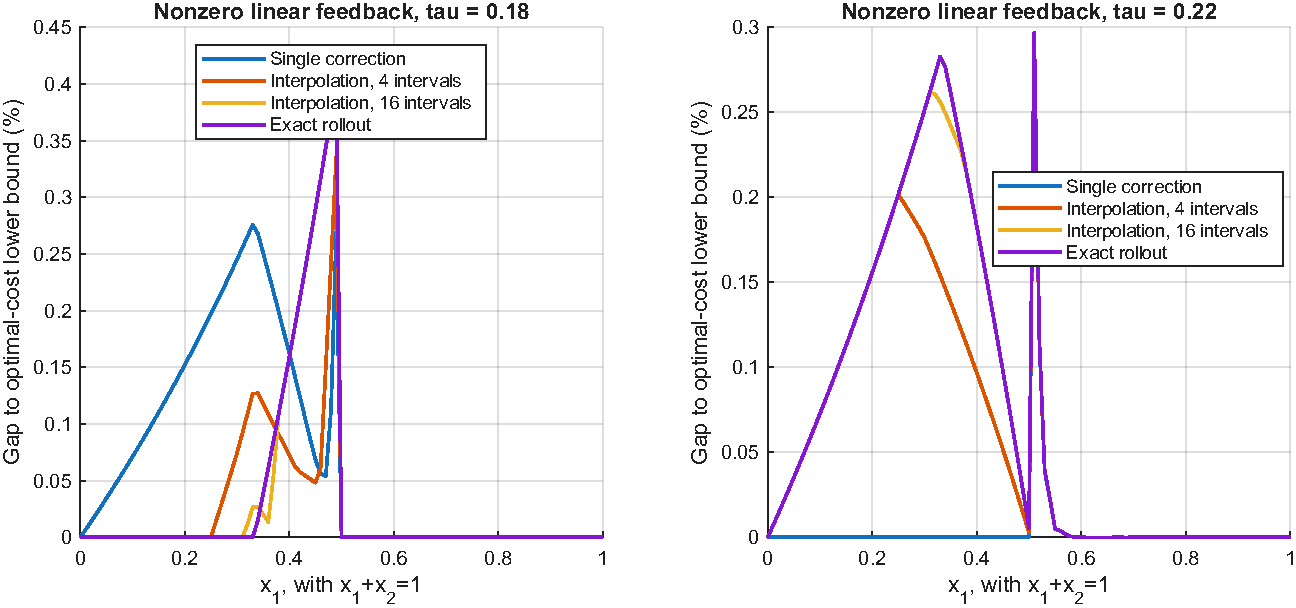
\includegraphics[width=\textwidth]{comparison_results/cost_comparison.pdf}
\caption{Total-cost gaps on the normalized two-resource problem in \eqref{eq:benchmark-data}. A smaller rollout-residual error does not imply a smaller total-cost gap.}
\label{fig:benchmark-cost}
\end{figure}

To examine sensitivity to dimension and small inventories, repeat \eqref{eq:benchmark-data} in $n/2$ independent pairs for $n\in\{2,4,8,16\}$. Use $w=\one$. The best linear feedback processes each inventory individually, with coefficient $p=(148/9)\one$. The single correction processes $\theta(x)$ coupled bundles in every pair, so its residual is $-9(n/2)\theta(x)$. Apply \eqref{eq:benchmark-interpolation} separately to each pair. Summing \eqref{eq:benchmark-interpolation-certificate} gives
\[
 R_p(x,\mu_M(x))\le-9\sum_{b=1}^{n/2}\min(x_{2b-1},x_{2b})
 \le-9(n/2)\theta(x).
\]
This proves feasibility and the same strict cost bound in every dimension tested. Summing \eqref{eq:benchmark-error} also preserves its error bound with $\one^\top x$ over all components. These examples are separable synthetic networks; they do not test general networks with operations connecting different pairs.

\begin{table}[htbp]
\centering
\begin{tabular}{rlrrr}
\hline
$n$ & Feedback & Uniform draws & Small inventories & One zero inventory\\
\hline
2 & Single correction & 17.726 & 7.059 & 0.000 \\ 
2 & Interpolation, $M=4$ & 17.693 & 7.037 & 0.000 \\ 
2 & Exact rollout & 17.680 & 7.032 & 0.000 \\ 
4 & Single correction & 10.300 & 0.523 & 0.000 \\ 
4 & Interpolation, $M=4$ & 20.287 & 3.570 & 13.028 \\ 
4 & Exact rollout & 20.264 & 3.568 & 13.015 \\ 
8 & Single correction & 7.254 & 0.027 & 0.000 \\ 
8 & Interpolation, $M=4$ & 20.966 & 3.701 & 17.263 \\ 
8 & Exact rollout & 20.950 & 3.698 & 17.247 \\ 
16 & Single correction & 3.675 & 0.002 & 0.000 \\ 
16 & Interpolation, $M=4$ & 20.401 & 4.329 & 18.979 \\ 
16 & Exact rollout & 20.384 & 4.327 & 18.963 \\ 
\hline

\end{tabular}
\caption{Mean cost reduction in percent from $K_{\rm lin}$ at $\tau=0.22$, over 80 initial states per column and dimension. All initial states have total inventory one.}
\label{tab:benchmark-scaling}
\end{table}

For Table~\ref{tab:benchmark-scaling}, the first group is formed by normalizing independent uniform draws on $(0,1)$. The second uses independent draws $10^{-6U}$ with $U$ uniform on $(0,1)$, then normalizes. The third sets one coordinate of each vector of uniform draws to zero before normalization, cycling through the coordinates. MATLAB's random seed is 271828. The single correction loses effectiveness with dimension and inventory imbalance. With a zero inventory it remains identically inactive along these trajectories, and its cost equals the linear cost. Interpolation and rollout can still use coupled operations in the other pairs.

\begin{table}[htbp]
\centering
\begin{tabular}{rrrrr}
\hline
$n$ & Single correction & Interpolation, $M=4$ & Explicit rollout & Online LP rollout\\
\hline
2 & 3.29 & 7.18 & 3.25 & 2299.50 \\ 
4 & 6.51 & 13.32 & 6.20 & 2235.95 \\ 
8 & 12.25 & 25.78 & 12.49 & 2656.65 \\ 
16 & 23.13 & 47.08 & 25.57 & 3724.20 \\ 
\hline

\end{tabular}
\caption{Median evaluation times in microseconds at $\tau=0.22$, measured in MATLAB R2025a on an AMD Ryzen 7 250 processor.}
\label{tab:benchmark-timing}
\end{table}

Table~\ref{tab:benchmark-timing} includes point location and scalar controller evaluation. Explicit times are medians of seven batches of 1200 evaluations; online LP times are medians of 12 solves of the original residual LP using \texttt{linprog}. Exact rollout is also evaluated by \eqref{eq:benchmark-rollout}, so the comparison includes an exact explicit implementation. Interpolation stores $2(M+1)$ floating-point values, shared by the identical pairs, and needs $M+1$ offline evaluations of \eqref{eq:benchmark-rollout}. Its intervals are uniform, so point location uses one division and integer indexing per pair. The single correction and exact rollout use their analytic formulas without a stored table. Offline table construction times and results for both values of $\tau$ are recorded with the experiment. These timings concern the supplied implementations; they do not establish optimized implementation limits or a general computational advantage. In particular, explicit rollout is competitive with the single correction on these separable examples.

The script \texttt{compare\_interpolation.m} reproduces the tables, figure, and numerical checks. Across the tests, the maximum constraint violation was $1.12\times10^{-16}$, the interpolation identity error was $1.12\times10^{-16}$, and the discrepancy between explicit rollout and independently solved residual LP objectives was $8.89\times10^{-16}$. No positive residual was observed. The feasibility and cost guarantees rely on \eqref{eq:benchmark-interpolation-certificate} and its sum over pairs; the numerical checks verify the implementation.

\section{Scope and research contribution}

The proposed result is the following alternative under Assumption~\ref{ass:data} and feasibility of \eqref{eq:synthesis}. Theorem~\ref{thm:synthesis} computes $p$ and a globally admissible stationary linear feedback of cost $p^\top x$ that is best in this class at every state. Theorem~\ref{thm:exactness} tests this cost against the unrestricted controls using \eqref{eq:interior-test}: zero certifies $J^*(x)=p^\top x$ at every state. If the minimum is negative, Theorem~\ref{thm:improvement} constructs \eqref{eq:improved-feedback}, whose cost is given by \eqref{eq:strict-gain} and is strictly smaller than that of every globally admissible stationary linear feedback at every strictly positive state. This is an exact decision and construction result, conditional on the stated feasibility assumption.

The ingredients have substantial precedents. Pates and Rantzer \cite[Theorem~2]{pates-rantzer} characterize when a conic control minimum is linear in the state; their first theorem gives an exact conic program under that property. Li and Bertsekas \cite{li-bertsekas} give DP results when linear Bellman closure holds. The restriction in \eqref{eq:restriction} has that property, and the iteration in Theorem~\ref{thm:best-linear} follows the established reasoning. Ohlin, Tegling, and Rantzer \cite{ohlin-tegling-rantzer} already solve positive network control with grouped input budgets by LP, and Arneson and Langbort \cite{arneson-langbort} already characterize optimal constant routing policies by LP for a continuous-time network class. Bellman-inequality lower bounds and policies are also established \cite{wang-odonoghue-boyd}. Accordingly, neither this iteration, synthesis in \eqref{eq:synthesis}, nor the test $q(p)\in G^\star$ is claimed as new in isolation.

The distinction from those exact linear-value results is that \eqref{eq:interior-test} examines only the computed coefficient $p$ and remains valid when the original Bellman operator lacks linear Bellman closure. The failed test leads to the explicit globally admissible feedback \eqref{eq:improved-feedback}. One-step rollout from $K_{\rm lin}$ obtains the same strict bound by minimizing the residual at every state \cite{li-johansson-martensson-bertsekas}. The difference from rollout is the particular formula in \eqref{eq:improved-feedback}: one offline minimizer at $w$ and conic decomposition give feedback with at most $n$ linear regions, evaluated without online optimization. When $G$ has the polyhedral form \eqref{eq:polyhedral}, rollout itself is a multiparametric LP and can also be compiled into explicit feedback \cite{bemporad-borrelli-morari}; no general computational advantage is established. Equation~\eqref{eq:rollout-comparison-costs} shows that neither feedback has lower total cost across all admissible problem data.

Proposition~\ref{prop:interpolation} settles the relation to feasible interpolation: the controller is exactly standard interpolation of rollout minimizers on \eqref{eq:interpolation-partition}, extended by positive homogeneity. Its region count and residual certificate are immediate consequences of that specialization, and Lemma~\ref{lem:verification} gives its strict cost bound. Thus neither the formula nor its cost certificate supplies an independent interpolation contribution. The adaptive algorithms of \cite{filippi-2004,bemporad-filippi-2006} need not choose this partition, but their interpolation step recovers the controller when supplied with these vertices.

The feasible approximate controllers in \eqref{eq:benchmark-interpolation} have an explicit residual-error bound and the same strict-improvement guarantee as $\mu$. Table~\ref{tab:benchmark-grid} shows that improved approximation of rollout does not monotonically improve total cost. Table~\ref{tab:benchmark-scaling} exposes the limitation of a correction controlled by the smallest inventory, and Table~\ref{tab:benchmark-timing} shows that exact explicit rollout is already competitive in evaluation time on the tested problems. These experiments give no general superiority result for $\mu$. They use independent resource pairs with nonzero linear feedback and do not establish performance on general coupled networks. Proposition~\ref{prop:resource} supplies the resource interpretation, while \eqref{eq:nonlinear-iterate} establishes failure of linear Bellman closure in a separate example.

Pates and Rantzer \cite{pates-rantzer} cover cones beyond the nonnegative orthant. The representation of $G_{\rm lin}$ in \eqref{eq:restriction} uses the orthant generators. Our cost comparison concerns globally admissible stationary linear feedbacks; it excludes controllers with internal memory and controllers required to be feasible only along their own trajectories. The interpolation specialization reduces the remaining novelty question to the combined synthesis and global optimality characterization under Assumption~\ref{ass:data}, especially the equivalence with testing one interior state when linear Bellman closure fails. Priority and publication significance of that combined characterization remain unestablished. The fixed-capacity networks in \cite{schurig-2026} fall outside the homogeneous constraints of Assumption~\ref{ass:data}.

\section*{Research tasks before submission}

This working checklist is to be removed from the submission version. Publication readiness depends primarily on establishing novelty and engineering relevance.

\begin{enumerate}
\item \textbf{Establish publication significance.}
Proposition~\ref{prop:interpolation} completes the specialization to the closest interpolation construction. Do not claim the controller formula or the interpolation-based strict cost bound as independent novelties. Assess the combined synthesis and one-interior-state optimality characterization against the exact positive-system results and general convex optimization. Check the earlier control construction of Gutman and Cwikel \cite{gutman-cwikel} beyond its available abstract if historical priority of interpolation is discussed. The current search does not establish priority for the remaining characterization.

\item \textbf{Identify a substantial engineering class.}
Develop a resource-conversion application with interacting inventories, operations requiring several resources, nonzero linear control options, and physically justified dynamics and costs. Establish when a globally admissible stationary linear feedback has finite cost; this assumption can exclude networks that require joint-resource operations to stabilize or empty. Identify useful applications where the assumption holds and coupled actions still offer substantial benefits. Explain the restrictions imposed by homogeneity, including the treatment of capacities and external arrivals. A scalable synthetic network may suffice; real data are not automatically necessary.

\item \textbf{Investigate behavior at boundary states.}
Table~\ref{tab:benchmark-scaling} quantifies the loss from empty and nearly empty inventories in independent pairs. Investigate corrections depending only on the resources needed by an operation when the operations overlap, and whether several corrections can be combined while retaining feasibility and a cost guarantee. The independent-pair construction in \eqref{eq:benchmark-interpolation} does not settle this question. Assess any additional novelty separately.

\item \textbf{Provide meaningful computational comparisons.}
Tables~\ref{tab:benchmark-grid}, \ref{tab:benchmark-scaling}, and \ref{tab:benchmark-timing} complete an initial comparison of nonzero linear feedback, $\mu$, feasible approximate explicit feedback, and exact rollout, including online LP and explicit evaluation. Extend the experiments to operations connecting different resource pairs and to approximation tolerances selected before construction. Report the cost of generic offline synthesis as well as evaluation, since the current benchmark has analytic rollout actions and shares identical tables between pairs. Preserve the residual and truncation checks in the supplied script.

\item \textbf{Audit proofs and numerical certificates.}
Check constraint cones with empty interior, boundary states, existence and attainment of minima, and the undiscounted case. Keep the controller comparison precise: globally admissible stationary linear feedbacks exclude controllers with internal memory and controllers required to be feasible only along their own trajectories. Verify numerical certificates with residual bounds consistent with the exact statements. Organize the submission around the main optimality-or-improvement result, supported by the computational formulas and engineering interpretation.
\end{enumerate}

The immediate priority is to assess the remaining optimality characterization and identify an engineering setting with overlapping coupled operations. The completed interpolation analysis and initial experiments do not justify a publication claim based on a new explicit controller or a general advantage over rollout.

\begin{thebibliography}{99}

\bibitem{rantzer-2022}
A. Rantzer.
\newblock Explicit solution to Bellman equation for positive systems with linear cost.
\newblock In \emph{Proceedings of the IEEE Conference on Decision and Control}, pages 6154--6155, 2022.
\newblock \url{https://doi.org/10.1109/CDC51059.2022.9993127}.

\bibitem{pates-rantzer}
R. Pates and A. Rantzer.
\newblock Optimal control on positive cones.
\newblock In \emph{Proceedings of the IEEE Conference on Decision and Control}, 2024.
\newblock Preprint: \url{https://arxiv.org/abs/2407.18774}.

\bibitem{li-rantzer}
Y. Li and A. Rantzer.
\newblock Exact dynamic programming for positive systems with linear optimal cost.
\newblock \emph{IEEE Transactions on Automatic Control}, 69(12):8738--8750, 2024.
\newblock \url{https://doi.org/10.1109/TAC.2024.3420716}.

\bibitem{li-bertsekas}
Y. Li and D. Bertsekas.
\newblock Semilinear dynamic programming: Analysis, algorithms, and certainty equivalence properties.
\newblock Preprint, arXiv:2501.04668v4, 2026.
\newblock \url{https://arxiv.org/abs/2501.04668v4}.

\bibitem{ohlin-tegling-rantzer}
D. Ohlin, E. Tegling, and A. Rantzer.
\newblock Optimal control of linear cost networks.
\newblock \emph{European Journal of Control}, 80:101068, 2024.
\newblock \url{https://doi.org/10.1016/j.ejcon.2024.101068}.

\bibitem{arneson-langbort}
H. Arneson and C. Langbort.
\newblock A linear programming approach to routing control in networks of constrained linear positive systems.
\newblock \emph{Automatica}, 48(5):800--807, 2012.
\newblock \url{https://doi.org/10.1016/j.automatica.2012.02.001}.

\bibitem{blanchini-2023}
F. Blanchini, P. Bolzern, P. Colaneri, G. De Nicolao, and G. Giordano.
\newblock Optimal control of compartmental models: The exact solution.
\newblock \emph{Automatica}, 147:110680, 2023.
\newblock \url{https://doi.org/10.1016/j.automatica.2022.110680}.

\bibitem{wang-odonoghue-boyd}
Y. Wang, B. O'Donoghue, and S. Boyd.
\newblock Approximate dynamic programming via iterated Bellman inequalities.
\newblock \emph{International Journal of Robust and Nonlinear Control}, 25(10):1472--1496, 2015.
\newblock \url{https://web.stanford.edu/~boyd/papers/adp_iter_bellman.html}.

\bibitem{de-farias-van-roy}
D. P. de Farias and B. Van Roy.
\newblock The linear programming approach to approximate dynamic programming.
\newblock \emph{Operations Research}, 51(6):850--865, 2003.
\newblock \url{https://doi.org/10.1287/opre.51.6.850.24925}.

\bibitem{li-johansson-martensson-bertsekas}
Y. Li, K. H. Johansson, J. M\aa rtensson, and D. P. Bertsekas.
\newblock Data-driven rollout for deterministic optimal control.
\newblock In \emph{Proceedings of the IEEE Conference on Decision and Control}, pages 2169--2176, 2021.
\newblock \url{https://arxiv.org/abs/2105.03116}.

\bibitem{bemporad-borrelli-morari}
A. Bemporad, F. Borrelli, and M. Morari.
\newblock Model predictive control based on linear programming---the explicit solution.
\newblock \emph{IEEE Transactions on Automatic Control}, 47(12):1974--1985, 2002.
\newblock \url{https://doi.org/10.1109/TAC.2002.805688}.

\bibitem{gutman-cwikel}
P.-O. Gutman and M. Cwikel.
\newblock Admissible sets and feedback control for discrete-time linear dynamical systems with bounded controls and states.
\newblock \emph{IEEE Transactions on Automatic Control}, 31(4):373--376, 1986.
\newblock \url{https://doi.org/10.1109/TAC.1986.1104270}.

\bibitem{filippi-2004}
C. Filippi.
\newblock An algorithm for approximate multiparametric linear programming.
\newblock \emph{Journal of Optimization Theory and Applications}, 120(1):73--95, 2004.
\newblock \url{https://doi.org/10.1023/B:JOTA.0000012733.44020.54}.

\bibitem{bemporad-filippi-2003}
A. Bemporad and C. Filippi.
\newblock Suboptimal explicit receding horizon control via approximate multiparametric quadratic programming.
\newblock \emph{Journal of Optimization Theory and Applications}, 117(1):9--38, 2003.
\newblock \url{https://cse.lab.imtlucca.it/~bemporad/publications/papers/jota-submpqp.pdf}.

\bibitem{bemporad-filippi-2006}
A. Bemporad and C. Filippi.
\newblock An algorithm for approximate multiparametric convex programming.
\newblock \emph{Computational Optimization and Applications}, 35(1):87--108, 2006.
\newblock \url{https://doi.org/10.1007/s10589-006-6447-z}.

\bibitem{jones-morari}
C. N. Jones and M. Morari.
\newblock Polytopic approximation of explicit model predictive controllers.
\newblock \emph{IEEE Transactions on Automatic Control}, 55(11):2542--2553, 2010.
\newblock \url{https://doi.org/10.1109/TAC.2010.2047437}.

\bibitem{rubagotti-2012}
M. Rubagotti, D. Barcelli, and A. Bemporad.
\newblock Approximate explicit MPC on simplicial partitions with guaranteed stability for constrained linear systems.
\newblock \emph{IFAC Proceedings Volumes}, 45(17):119--125, 2012.
\newblock \url{https://doi.org/10.3182/20120823-5-NL-3013.00014}.

\bibitem{hertneck-2018}
M. Hertneck, J. K\"ohler, S. Trimpe, and F. Allg\"ower.
\newblock Learning an approximate model predictive controller with guarantees.
\newblock \emph{IEEE Control Systems Letters}, 2(3):543--548, 2018.
\newblock \url{https://doi.org/10.1109/LCSYS.2018.2843682}.

\bibitem{chakrabarty-2019}
A. Chakrabarty, R. Quirynen, C. Danielson, and W. Gao.
\newblock Approximate dynamic programming for linear systems with state and input constraints.
\newblock In \emph{Proceedings of the European Control Conference}, 2019.
\newblock \url{https://doi.org/10.23919/ECC.2019.8795815}.

\bibitem{wang-boyd-2011}
Y. Wang and S. Boyd.
\newblock Fast evaluation of quadratic control-Lyapunov policy.
\newblock \emph{IEEE Transactions on Control Systems Technology}, 19(4):939--946, 2011.
\newblock \url{https://doi.org/10.1109/TCST.2010.2056371}.

\bibitem{ganguly-2025}
S. Ganguly and D. Chatterjee.
\newblock Explicit feedback synthesis driven by quasi-interpolation for nonlinear model predictive control.
\newblock \emph{IEEE Transactions on Automatic Control}, 70(7):4751--4758, 2025.
\newblock \url{https://doi.org/10.1109/TAC.2025.3538767}.

\bibitem{rahal-2025}
S. S. Rahal, Z. Li, D. J. Papageorgiou, and A. AlShammari.
\newblock Decision rule-based method for multiparametric linear programming.
\newblock \emph{Computers \& Chemical Engineering}, 199:109157, 2025.
\newblock \url{https://doi.org/10.1016/j.compchemeng.2025.109157}.

\bibitem{ohlin-rantzer-tegling}
D. Ohlin, A. Rantzer, and E. Tegling.
\newblock Heuristic search for linear positive systems.
\newblock \emph{Automatica}, 192:113153, 2026.
\newblock \url{https://doi.org/10.1016/j.automatica.2026.113153}.

\bibitem{schurig-2026}
R. Schurig, D. Ohlin, A. Rantzer, E. Tegling, and R. Findeisen.
\newblock Model predictive control for constrained linear positive systems on graphs.
\newblock \emph{IEEE Control Systems Letters}, 10:481--486, 2026.
\newblock \url{https://doi.org/10.1109/LCSYS.2026.3698436}.

\bibitem{mehrivash-shafiei}
H. Mehrivash and M. H. Shafiei.
\newblock Constrained model predictive control for positive systems.
\newblock \emph{IET Control Theory \& Applications}, 13(10):1491--1499, 2019.
\newblock \url{https://doi.org/10.1049/iet-cta.2018.5755}.

\bibitem{bertsekas}
D. P. Bertsekas.
\newblock \emph{Dynamic Programming and Optimal Control, Volume II}.
\newblock Athena Scientific, 3rd edition, 2007.

\bibitem{boyd-vandenberghe}
S. Boyd and L. Vandenberghe.
\newblock \emph{Convex Optimization}.
\newblock Cambridge University Press, 2004.

\end{thebibliography}
\end{document}
